% !TEX TS-program = pdflatex
% !TEX encoding = UTF-8 Unicode

% This is a simple template for a LaTeX document using the "article" class.
% See "book", "report", "letter" for other types of document.

\documentclass[11pt]{article} % use larger type; default would be 10pt

\usepackage[utf8]{inputenc} % set input encoding (not needed with XeLaTeX)

%%% Examples of Article customizations
% These packages are optional, depending whether you want the features they provide.
% See the LaTeX Companion or other references for full information.

%%% PAGE DIMENSIONS
\usepackage{geometry} % to change the page dimensions
\geometry{a4paper} % or letterpaper (US) or a5paper or....
% \geometry{margin=2in} % for example, change the margins to 2 inches all round
% \geometry{landscape} % set up the page for landscape
%   read geometry.pdf for detailed page layout information

\usepackage{graphicx} % support the \includegraphics command and options

% \usepackage[parfill]{parskip} % Activate to begin paragraphs with an empty line rather than an indent

%%% PACKAGES
\usepackage{booktabs} % for much better looking tables
\usepackage{amssymb}
\usepackage{amsthm}
\usepackage{amsmath}
\usepackage{dsfont}
\usepackage{listings}
\usepackage{pgfplots,tikz}
\usepgfplotslibrary{fillbetween}
\pgfplotsset{compat=1.15}
\usepackage{array} % for better arrays (eg matrices) in maths
\usepackage{paralist} % very flexible & customisable lists (eg. enumerate/itemize, etc.)
\usepackage{verbatim} % adds environment for commenting out blocks of text & for better verbatim
\usepackage{subfig} % make it possible to include more than one captioned figure/table in a single float
% These packages are all incorporated in the memoir class to one degree or another...

%%% HEADERS & FOOTERS
\usepackage{fancyhdr} % This should be set AFTER setting up the page geometry
\pagestyle{fancy} % options: empty , plain , fancy
\renewcommand{\headrulewidth}{0pt} % customise the layout...
\lhead{}\chead{}\rhead{}
\lfoot{}\cfoot{\thepage}\rfoot{}

%%% SECTION TITLE APPEARANCE
\usepackage{relsize}
\usepackage{sectsty}
\allsectionsfont{\mdseries\upshape\larger} % (See the fntguide.pdf for font help)
% (This matches ConTeXt defaults)

%%% ToC (table of contents) APPEARANCE
\usepackage[nottoc,notlof,notlot]{tocbibind} % Put the bibliography in the ToC
\usepackage[titles,subfigure]{tocloft} % Alter the style of the Table of Contents
\renewcommand{\cftsecfont}{\rmfamily\mdseries\upshape}
\renewcommand{\cftsecpagefont}{\rmfamily\mdseries\upshape} % No bold!

\theoremstyle{definition}
\newtheorem{theorem}{Theorem}[section]
\newtheorem{definition}[theorem]{Definition}
\newtheorem{lemma}[theorem]{Lemma}
\newtheorem*{example}{Example}

\theoremstyle{remark}
\newtheorem*{remark}{Remark}

\newcommand{\ZZ}{\mathbb{Z}}
\newcommand{\RR}{\mathbb{R}}
\newcommand{\code}[1]{\texttt{#1}}
\newcommand{\myspan}[1]{\textrm{span} \lbrace {#1} \rbrace}
\newcommand{\stab}[2]{\textrm{Stab}_{#1}({#2})}

%%% END Article customizations

%%% The "real" document content comes below...

\title{Optimization Topics Report}
\author{Joshua Gunter\\  Daniel Snider}
%\date{} % Activate to display a given date or no date (if empty),
         % otherwise the current date is printed 

\begin{document}

\maketitle

\tableofcontents

%% INTRODUCTION
\section{Introduction}

Linear programming is a method of mathematical optimization, where the goal is to find the optimal value of a linear objective function over a set of variables, which are constrained by a set of linear inequalities. If all the variables must also be integers, then the problem is referred to as an integer program. While linear programs may be efficiently solved with the use of algorithms such as the Simplex Method, there is no reliably fast method for integer programming problems. In fact, they have been proven to be NP-Hard. Because of this, better methods and algorithms for solving integer programs is an active field of research.

In this study, we investigated a method to speed up the solving of a special set of symmetric integer programs. An integer program (hereafter referred to as an IP) has symmetry if the value of its objective function is invariant under permutations of the coordinate axes. More plainly, swapping around the entries of a vector $v$ describing the solution to an IP doesn't change the value of $f(v)$, where $f$ is the objective function.

When an IP is symmetric in this way we can find a set of orthogonal subspaces in $\mathbb{R}^n$, at least one of which any optimal solution must lie "close to". We can therefore restrict the search space for the optimum by setting up quadratic bounds, restricting how far away an answer can be from the aforementioned subspaces. Exactly how "close to" one of these subspaces the solution has to be is not yet known. The goal of this project is to experimentally test different possible bounds and discover what the effect of adding these bounds are on the runtime of solving IPs using standard solvers. In general, it is expected that with a tighter bound, the solver should be able to find a solution faster than with a looser bound, as there is less space to search through. By experimentally checking various bounds, we can determine whether or not this strategy would be useful once methods to find an exact bound are discovered.

This report consists of four main sections. First are definitions of terms from linear programming, group theory, and geometry required as background. Second we look at the algorithms and methods used to construct special subspaces and integer programs, and compute the additional quadratic constraints. Third we list some of the computational results found. Finally, we give some comments and recommendations for future work.

%% DEFINITIONS
\section{Background}

\subsection{Linear and Integer Programming}

In order to motivate the discussion in this report, we first need to define what exactly linear and integer programming is.

\begin{definition}[Linear Program]
A linear programming problem is a mathematical optimization problem of the form
\begin{align*}
&\max{} \ c^\intercal x \\
&\textrm{s.t. } Ax \leq b, \\
&\textrm{and } x \geq 0
\end{align*}

Where $c, x, b \in \RR^n, A \in \RR^{m \times n}$. 
\end{definition}

 Described more geometrically, we want to find the maximum value of a linear function $f(x) = c^\intercal x$ over the intersection of the two sets of halfspaces $Ax \leq b$ and $x \geq 0$  in $\RR^n$. The space of possible solutions is known as the feasible region. If the feasible region is the empty set $\emptyset$, then the linear program is denoted as infeasible. There are fast algorithms for solving these problems such as the Simplex Method and Interior Point methods, and many different problems that may be modelled through linear programs. 
	For a simple example of a linear program, consider the problem
\begin{align*}
&\max{ x_1 + x_2 }, \ \textrm{subject to} \\
&-3x_1 + 5x_2 \leq 8 \\
&3x_1 + x_2 \leq 10 \\
&x_1, x_2 \geq 0
\end{align*}

Since this problem is only 2 dimensional, we can graph the inequalites and feasible region and find the solution by inspection:
\begin{figure}[h]
\centering
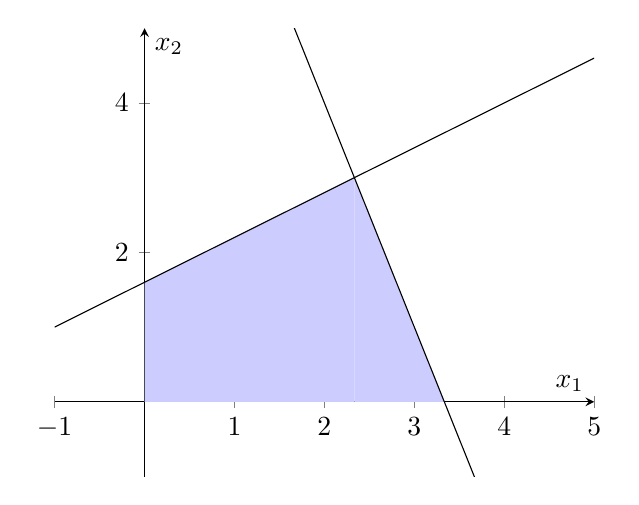
\begin{tikzpicture}
 \begin{axis}[
	thick, smooth,
	ymin = -1, ymax = 5, xmin = -1, xmax = 5,
	axis lines = middle,
	xlabel = $x_1$, ylabel = $x_2$
	]
	\addplot [domain=-1:5, name path = one] {3/5*x + 8/5};
	\addplot [domain=-1:5, name path = two] {-3*x + 10};
	\path[name path=xaxis] (0,0) -- (5,0);
	\addplot[blue!20] fill between[of=one and xaxis, soft clip = {domain=0:2.333}];
	\addplot[blue!20] fill between[of=two and xaxis, soft clip = {domain=2.332:3.3333}];
 \end{axis}
\end{tikzpicture}
\end{figure}

It can be seen that the point $x_1 = 7/3, x_2 = 3$ lying on the intersection of the two lines will be the optimal solution to this linear program. Note that for any linear program in $n$ dimensions, an optimal solution will satisfy $n$ of the constraints with equality. This is an important property of linear programs, and is what allows solvers to be able to find solutions for them rapidly.

\begin{definition}[Integer Program]
An integer programming problem is a linear program with the additional constraint that the solutions $x$ must lie within $\ZZ^n$. In other words, it is of the form
\begin{align*}
&\max{} \ c^\intercal x \\
&\textrm{s.t. } Ax \leq b, \\
& x \geq 0, \\
& x \in \ZZ^n
\end{align*}
\end{definition}

While integer programs may seem to be quite similar to linear programs, they are much harder. In fact, they are NP-hard: solving an integer program can be shown to be equivalent to NP-Hard problems from graph theory, such as minimum vertex cover or the travelling salesman problem. For a general understanding of why this is the case, consider the same linear program as in the previous example with added integrality constraints:
\begin{figure}[h]
\centering
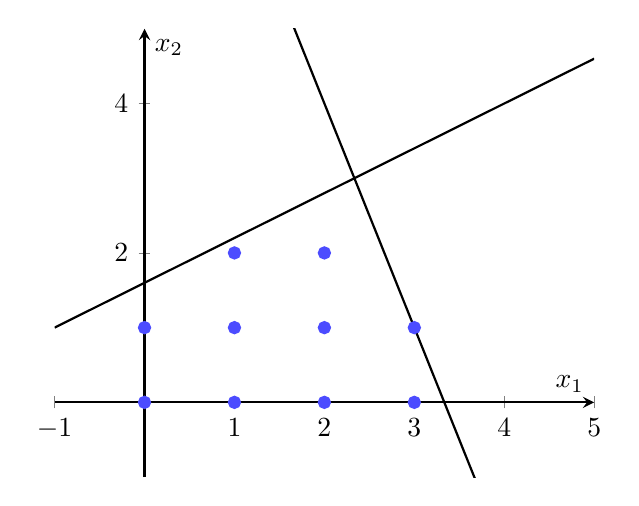
\begin{tikzpicture}
 \begin{axis}[
	thick, smooth,
	ymin = -1, ymax = 5, xmin = -1, xmax = 5,
	axis lines = middle,
	xlabel = $x_1$, ylabel = $x_2$
	]
	\addplot [domain=-1:5, name path = one] {3/5*x + 8/5};
	\addplot [domain=-1:5, name path = two] {-3*x + 10};
	\foreach \n in {0, ..., 3}{
		\foreach \m in {0,...,1}{
			\addplot [mark=*, blue!70] coordinates {(\n,\m)};
		}
	}
	\addplot [mark=*, blue!70] coordinates {(1,2)};
	\addplot [mark=*, blue!70] coordinates {(2,2)};
	\path[name path=xaxis] (0,0) -- (5,0);
 \end{axis}
\end{tikzpicture}
\end{figure}

In this case, we end up with two optimal solutions: $x = (2,2)$ and $x = (3,1)$. Note that $(2,2)$ does not lie on the boundary of the feasible region of the original LP. In an integer program,  we have no guarantee of this like we do with a linear program. This property is what makes integer programs hard. The standard solving strategy for an integer programming typically consists of solving the LP relaxation, which is the IP without integrality constraints, and then checking if there is an integer solution. If not, we make two new LPs with additional constraints to cut out the space containing non-integral optimal solutions, and recursively solve this in the same manner.

\subsection{Groups and their Representations}

\subsubsection{Groups}

Group Theory is a fundamental area in the field of abstract algebra which studies algebraic structures with symmetry. As we are studying integer programs that contain underlying symmetry, group theory is naturally heavily involved in the mathematics behind the algorithms implemented. In this section, we aim to give a crash course in the group theory involved. For additional resources on this topic, we recommend texts such as \cite{grouptext} or \cite{algebra}.

\begin{definition} [Group]
A group is an algebraic structure $(G,*)$ consisting of a set $G$ and an operation $* : G \times G \to G$ satisfying the group axioms. These are as follows:
\begin{description}
\item[Closure:] For all $x,y \in G$, $x*y \in G$.
\item[Associativity:] For all $x,y,z \in G$, $x*(y*z) = (x*y)*z$.
\item[Identity:] There exists an element $e \in G$ such that $e*g = g*e = g$ for all $g \in G$.
\item[Inverse:] For all $g \in G$, there exists a $g^{-1} \in G$ such that $g*g^{-1} = g^{-1}*g = e$.
\end{description}
\end{definition}

\begin{example}
Consider the set of integers with addition, $(\ZZ, +)$. Based on the properties of addition, it is easily seen that this is a group. Closure is satisfied because any integer plus another integer yields an integer. Associativity is one of the properties of addition. The number $0$ satisfies the properties of the identity element, as $0 + z = z + 0 = z$ for all integers $z$. The final axiom existence of an inverse is also satisfied, as $z + (-z) = (-z) + z = 0$ for all $z$.
\end{example}

\begin{example}
For another basic example, consider $(\mathbb{Q} \setminus \lbrace 0 \rbrace, *)$, the set of rational numbers with 0 removed under the operation of multiplication. The first two axioms hold trivially from the definition of multiplication on rational numbers, the element 1 serves as identity, and every non-zero rational number $q$ has a multiplicative inverse $1/q$. Note that the inverse axiom is what forces us to use $\mathbb{Q} \setminus \lbrace 0 \rbrace$ as the underlying set rather than $\mathbb{Q}$, as 0 has no inverse element.
\end{example}

\begin{example}
The most important example of groups in the context of this paper are permutation groups. Let $S_n$ be the set of permutations of $n$ elements, with the operation being composition of functions $\circ$. For any two permutations $\pi, \sigma \in S_n$, $\pi \circ \sigma$ is also a permutation, so $S_n$ is closed. For any three permutations $\pi, \sigma, \gamma \in S_n$, $((\pi \circ \sigma) \circ \gamma)(x) = (\pi \circ \sigma)(\gamma(x)) = \pi (\sigma(\gamma(x))) = \pi((\sigma \circ \gamma)(x)) = (\pi \circ (\sigma \circ \gamma))(x)$, therefore composition of permutations is associative. The identity permutation $e$ which maps every element to itself serves as identity, and for any permutation we can find another permutation reversing it. Therefore $(S_n, \circ)$ is a group.
\end{example}

In this project, all examples of groups we deal with are permutation groups which are subgroups of $S_n$.

\begin{definition}[Subgroup]
A subgroup $H$ of a group $G$ is a subset of the elements of $G$ such that the group axioms still hold. We denote this by $H \leq G$.
\end{definition}

Another important concept required are group actions.

\begin{definition}[Group Action]
Let $G$ be a group, and $X$ be a set. A group action is a function $\phi : G \times X \to X$, satisfying the two group action axioms:
\begin{description}
\item[Identity:] Let $e \in G$ be the identity element of the group. $\phi(e,x) = x$ for all $x \in X$.
\item[Compatibility:] For all $g, h \in G$, $\phi(gh, x) = \phi(g, \phi(h, x))$ for all $x \in X$.
\end{description}
When working with group actions, it is common to write the action of a group on an element of a set as an operation $g \cdot x$ rather than using function notation.
\end{definition}

A group action may be categorized as being "transitive". In this report, we will only deal with groups that have transitive group actions.

\begin{definition}[Transitive]
A group $G$ acts transitively on a set $X$ if for all $x,y \in X$, there exists a $g \in G$ such that $g \cdot x = y$.
\end{definition}

When we consider the action of a group on a set, there are two structures that are of particular interest to us, namely the orbit of an element under a group action and the stabilizer subgroup with respect to an element.

\begin{definition}[Orbit]
Let $G$ be a group, and let $X$ be a set acted upon by $G$. The orbit of an element $x \in X$ is the set $\lbrace g \cdot x \ | \ g \in G \rbrace$, consisting of elements of $X$ that $x$ can be moved to by elements of $G$. This is a subset of $X$, and is denoted by $G \cdot x$ or $Gx$. The set of all orbits $G \cdot X$ is a partition of $X$.
\end{definition}

\begin{definition}[Stabilizer]
Let $G$ be a group. The stabilizer of $G$ with respect to $x \in X$ is defined as the set $\stab{G}{x} = \lbrace x \in X \ | \ gx = x\rbrace$ of elements in $G$ fixing $x$. This is a subgroup of $G$.
\end{definition}

We can now define the specific subset of permutation groups that we are working with.

\begin{definition}[Primitive Groups]
Let $G \leq S_n$ be a permutation group acting on a set $X \neq \emptyset$. $G$ is primitive if it acts transitively on $X$ and preserves no non-trivial partition of $X$. This means that for all $x \in X$, the orbit $G \cdot x = \lbrace x \rbrace$ or $G \cdot x = X$.
\end{definition}

We have now finished defining all group theoretic terms required for the rest of this report.

\subsubsection{Group Representations}

In order to perform computations with groups, we require ways to represent them and how they act numerically. This is where the Representation Theory of groups comes in. Using representation theory, we can transform group computations into linear algebra computations, which computers excel at. We will start off with the basic definition of a representation of a group.

\begin{definition} [Representation]
Let $G$ be a group and $V$ a vector space over a field $F$. A representation of $G$ in $V$ is a homomorphism $\rho : G \to GL(V)$, where $GL(V)$ denotes the group of automorphisms of $V$ (this usually corresponds to the group of invertible $n \times n$ matrices with entries in $F$). In other words, a representation is function preserving the relations between elements of $G$: for all $g, h \in G$, $\rho(gh) = \rho(g)\rho(h)$. This property also implies that $\rho$ preserves identity and inverse, as $\rho(e)\rho(g) = \rho(eg) = \rho(g)$, and $\rho(e) = \rho(gg^{-1}) = \rho(g)\rho(g^{-1}$. When $\rho$ is given, we say that $V$ is a representation space of G (or simply a representation of G).
\end{definition}

Representations may be either reducible or irreducible. A representation $\rho$ is reducible if there exists a subspace $W$ of $V$ such that $\lbrace 0 \rbrace \neq W \subset V$ which is invariant under the action of $\rho(G)$. That is for all $g \in G$ and $w \in W$, $\rho(g)w \in W$. In this case $W$ is called an invariant subspace of $G$, and we can define a subrepresentation of $\rho$ \ $\rho|_W : G \to GL(W)$ by restricting the action of $\rho$ to $W$:

\[ \rho|_W(g) = \begin{cases}
	\rho(g) & \textrm{if } \rho(g) \in W \\
	0 & \textrm{otherwise}
	\end{cases}
\]

If $\rho$ does not have any invariant subspaces, then $\rho$ is irreducible. On the other hand, if there is a decomposition of $\rho$ into a direct sum of irreducible subrepresentations $\rho = \rho_1 \oplus \rho_2 \oplus ... \oplus \rho_k$, then $\rho$ is called completely reducible. Due to Maschke's Theorem in representation theory, we know that every representation of finite groups mapping from $G \to GL_n(\mathbb{C})$ is completely reducible (Mashke's Theorem is actually a little more general, but for our purposes all we'll need are representations of groups as complex matrices). These decompositions of representations into subrepresentations correspond decompositions of $V$ into a direct sum

\[ V = V_1 \oplus V_2 \oplus ... \oplus V_k \]

of invariant subspaces. This fact will be incredibly important for much of our work.

\begin{example} 
Consider the cyclic permutation group $C_3 = \lbrace (), (123), (132) \rbrace$. We can represent the elements of $C_3$ as matrices in $GL_3(\mathbb{C})$ using the representation
\[ \rho(()) = \begin{bmatrix}
	1 & 0 & 0 \\
	0 & 1 & 0 \\
	0 & 0 & 1
	\end{bmatrix},
\rho((123)) = \begin{bmatrix}
	0 & 0 & 1 \\
	1 & 0 & 0 \\
	0 & 1 & 0
	\end{bmatrix},
\rho((132)) = \begin{bmatrix}
	0 & 1 & 0 \\
	0 & 0 & 1 \\
	1 & 0 & 0
	\end{bmatrix}.
\]
We can then examine how $G$ permutes the coordinates of vectors in $\mathbb{C}^3$ by performing matrix-vector multiplication with the elements of $\rho(G)$.
\end{example}

For all group representations $\rho(G) \leq GL_n(F)$, there is a specific special invariant subspace where $G$ not only keeps vectors within the subspace, but also preserves the vectors exactly. We denote this as the fixed space,

\[ \textrm{Fix}(G) = \lbrace x \in F^n \ | \ g \cdot x = x \rbrace \]. 

In the case of transitive groups, $\textrm{Fix}(G) = \myspan{\mathds{1}}$.

\subsection{Convex Geometry}

As the feasible region of a linear program is a convex set, linear programming and convex geometry are closely related. In this section, we will define what exactly it means for a set to be convex, and a convex geometric object that we will be working with frequently.

\begin{definition}[Convexity]
A set of points $S$ is convex if for any two points $p, q \in S$, the line between $p$ and $q$ is contained in $S$. More formally, for all $p, q \in S$, for all $t \in [0, 1]$, $tp + (1-t)q \in S$.
\end{definition}

Alternatively, we could also charactize as convex set as being a set containing all convex combinations of any subset of points within the set.

\begin{definition}[Convex Combination]
A convex combination of a set of points $\lbrace p_1, p_2, ..., p_k \rbrace$ is a linear combination

\[ \sum_{i = 1}^{k} \lambda_i p_i, \quad \textrm{where } \lambda_i \geq 0, \ \sum_{i=1}^{k} \lambda_i = 1. \]

\end{definition}

In this report, we are primarily concerned with a specific type of convex object, namely the orbit polytope of a group.

\begin{definition}[Orbit Polytope]
Let $G \leq S_n$ be a permutation group, acting on vectors by permuting their entries. The orbit polytope of a point $x \in \RR^n$ is the convex hull of the orbit $Gx$, denoted $\textrm{conv}(Gx)$. In other words, it is the set of all convex combinations of permutations of $x$ by $G$.
\end{definition}

\begin{example} Consider the symmetric group $S_3$ acting on the point $x = (1, 0, 0) \in \RR^3$. Its orbit is $S_3 x = \lbrace (1, 0, 0), (0, 1, 0), (0, 0, 1) \rbrace$, and its orbit polytope is the convex hull of these three points, which describes a surface in $\RR^3$:

\begin{figure}[h]
\centering
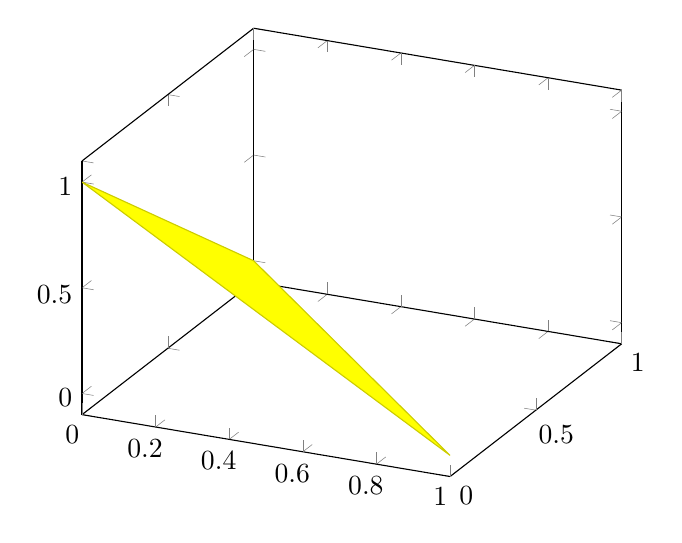
\begin{tikzpicture}
\begin{axis}
\addplot3[
   patch,
  patch type=triangle
]  coordinates {
	(1,0,0)  (0,1,0)  (0,0,1)
};
\end{axis}
\end{tikzpicture}
\end{figure}
\end{example}

% CORE POINTS
\subsection{Core Points}

In this section, we will be looking at the definition of what a core point is, and how they relate integer programs. These objects were first studied by \cite{some} while researching the geometrical aspects of symmetric integer programs.

\begin{definition}[Core Point]
A core point of a permutation group $G$ is a point $z \in \mathbb{Z}^n$ such that the orbit polytope $\textrm{conv}(Gz)$ contains no interior integer points. In other words, $\textrm{conv}(Gz) \cap \mathbb{Z}^n = Gz$. The set of all core points of $G$ is called the \textbf{core set} and is denoted by $\textrm{core}(G)$.
\end{definition}

A very important result from \cite{rehn} is that these core points must lie "close to" the invariant subspaces of their group $G$. The proof of this is rather technical, so rather than give the full theorem and proof we will sketch out the general idea behind it. First, we define a function $\mu : \ZZ^n -> \RR$ which maps points $z \in \ZZ^n$ to the minimal distance of a point in the affine hull of $Gz$ from the fixed space $\textrm{Fix}(G)$. We then construct a minimal bounding ellipsoid $E$ around the orbit polytope $\textrm{conv}(Gz)$, where $z \in \textrm{core}(G)$, using results from Theorem 2.2 in \cite{barvinok/blekherman}. We then find a scaled and translated ellipsoid $E'$ constructed from $E$ such that $E' \subseteq \textrm{conv}(Gz)$, and use this to find conditions for when $E'$ (and by extension $\textrm{conv}(Gz)$ contain interior integer points. From this exploration we can find a constant bound $C(G)$ for the projection of $z$ onto any of the invariant subspaces of $G$, such that $z \in \textrm{core}(G) \implies  ||z|_{V_i}|| \leq C(G)$. If $||z|_{V_i}|| \geq C(G)$, then $E' \subseteq \textrm{conv}(Gz)$ will contain an integer point inside of it, and therefore $z$ can not be a core point.

A natural question is what these points have to do with solving integer programs. Before that question can be answered, let us state the precise definition of a symmtery of an integer programming problem. 

\begin{definition}[IP Symmetry]
A \textbf{symmetry} of an integer program with a feasible region $P \subset \RR^n$ and objective function $f : \ZZ^n \rightarrow \RR$ is a permutation $g \in S_n$ such that $gx \in P$ and $f(x) = f(gx)$ for all $x \in P$. The group of all these permutations is the symmetry group $G \leq S_n$ of the integer program.
\end{definition}

Now we can state the result connecting these two concepts of core points and integer programs, Theorem 7.3 from \cite{rehn}.

\begin{theorem} \label{cpclose}
Let $\min_{x \in C \cap \ZZ^n} f(x)$ be a convex integer optimization problem, with a convex function $f$ and a convex set $C \subseteq \mathbb{R}^n$ and a symmetry group $G$. Then $\min_{x \in C \cap \ZZ^n} f(x) = \min_{x \in C \cap \textrm{core}(G)} f(x)$.
\end{theorem}

The idea behind the proof of this theorem is that if the optimal solution $x \in C \cap \ZZ^n$ is not a core point, then we can find some integral points inside of $\textrm{conv}(Gx)$. By choosing an $x'$ from within the integer points $\textrm{conv}(Gx) \cap \ZZ^n$ that has minimal norm, we are guaranteed that $x'$ is a core point for $G$. Since $x' \in \textrm{conv}(Gz)$, $x'$ is a convex combination of permutations of $x$, so $x' = tx + (1-t)(gx)$ for some $t \in [0,1], g \in G$. Because $f$ is convex, $f(tx + (1-t)(gx)) \leq tf(x) + (1-t)f(gx) \implies f(x') \leq f(x)$, as $f(x) = f(gx)$. Therefore $x'$ is an optimal solution for the integer program with $x' \in \textrm{core}(G)$.

Due to this theorem, we can find an optimal solution to any integer program with a symmetry by only looking at the core points of the symmetry group. In some cases, there are a finite number of core points, and we can devise algorithms based on enumerating core points and searching for an optimal solution. However in this project we focused on a set of groups containing infinite core points, in which case enumeration of core points won't help us any. Instead, armed with our additional constraints on the norm of the projection of core points on the invariant subspaces of the group, we can restrict the size of the feasible region when searching for solutions to the integer program. This is the extent of the knowledge we will need about core points for this project.

%% METHODS
\section{Methods \& Algorithms}

Now that we know that we can add additional constraints to reduce the size of the feasible region, all we need are algorithms to actually compute all the required data. First, we will examine two methods to construct invariant subspaces of symmetry groups, one method using information from character theory, the second using results about group actions in relation to invariant subspaces. Next, we will look at how we can actually compute a set of core points of group, and use these to construct difficult integer programs to test the effectiveness of this method on. Finally, we will cover how to compute the new quadratic constraints that we can use to solve these problems faster.

% INVARIANT SUBSPACES
\subsection{Computing Invariant Subspaces}

% METHOD 1
\subsubsection{Irreducible Characters} \label{charmethod}

This method was the primary one used during the project, and makes use of results found in character theory. Many formulas dealing with representations of groups can be transformed into formulas involving their characters, which are much easier to work with computationally.

\begin{definition}[Character] 
The \textbf{character} $\chi_\rho : G \rightarrow \mathbb{C}$ of a representation $\rho : G \rightarrow GL_n(\mathbb{C})$ is defined as $\textrm{tr}(\rho(g))$ for all $g \in G$.
\end{definition}

Similarly to how representations can be decomposed into a direct sum of irreducible representations, the character of a representation can be decomposed into a linear combination of irreducible characters. This means we can write any character of a group G as

	$$ \chi = m_1\chi_1 + m_2\chi_2 + ... + m_k\chi_k, $$

where $m_i \in \mathbb{Z}_{\geq 0}$, and $\chi_i$ is the character of the $i$th irreducible representation of $G$. We can compute each $m_i$ by taking an inner product of the characters, using the formula:

\begin{equation}
m_i = \frac{1}{|G|} \sum_{g \in G} \chi_i(g) \chi(g^{-1}).
\end{equation}

From this, we can see that as long as we know the values of the irreducible characters, we can easily compute what the decomposition is for any character.

The decomposition of a character $\chi$ into a sum of irreducible characters corresponds to the decomposition of the related representation $\rho$ into a direct sum of subrepresentations. We can rewrite $\rho$ into

	$$ \rho = \rho_1^{(m_1)} \oplus \rho_2^{(m_2)} \oplus ... \rho_k^{(m_k)}. $$

Each of these subrepresentations $\rho_i^{(m_i)}$ corresponds to an invariant subspace $V_i$, which is what we're really interested in. In \cite{char}, we can find the following formula for the projection of $\mathbb{C}^n$ onto $V_i$:

\begin{equation} \label{eq:projection}
P_i = \frac{m_i\chi_i(1)}{|G|} \sum_{g \in G} \chi_i(g^{-1})\rho(g).
\end{equation}

The column space of $P_i$ is then a basis for $V_i$. At this point we have all of the basic tools necessary for computation of invariant subspaces. However these formulas do have a weakness: as they require summing over the all of the group elements, the runtime required can be exorbitant for larger groups. We can make our lives a little easier by doing some computations with conjugacy classes of groups, along with a couple of additional small optimizations.

\begin{definition}[Conjugacy Classes]
For a group $G$, two elements $a, b \in G$ are said to be \textbf{conjugate} if $a = gbg^{-1}$ for some $g \in G$. A \textbf{conjugacy class} is a subset of $G$ containing elements that conjugate with one another. The conjugacy class containing an element $g \in G$ is denoted by $Cl(g)$.
\end{definition}

This relation can easily be seen to be reflexive, symmetric, and transitive, and is therefore an equivalence relation. As such, we can partition $G$ in a set of disjoint conjugacy classes. This is very useful to us because characters are constant over a conjugacy class, so by dealing with conjugacy classes we can avoid computations summing over every group element. Instead we can sum over the conjugacy classes whenever we are only dealing with characters. We can perform an additional optimization making use of the fact that $\chi(g^{-1}) = \overline{\chi(g)}$, where $\overline z$ denotes the complex conjugate of $z \in \mathbb{C}$. This allows us to compute $\chi(g^{-1})$ without needing to know what $g^{-1}$ actually equals. We can now re-express the previous formula for computing the coefficients of the irreducible characters in the decomposition of a character by

\begin{equation} \label{eq:chars}
m_i = \frac{1}{|G|} \sum_{Cl(g) \subseteq G} |Cl(g)| \chi_i(g) \overline{\chi(g)}.
\end{equation}

This is the equation we will actually be implementing. Unfortunately as for the second part of finding invariant subspaces, computing the projection matrices $P_i$, due to the fact that the representation itself is being used in the formula we will not be able to make use of conjugacy classes to save time, as representations are definitely not constant over conjugacy classes.

All of these computations were performed using GAP, which has excellent support for computations with characters. Character tables containing information about characters of a group $G$ can be obtained with the function \code{CharacterTable(G)}, with the values for all irreducible characters of a group found in the attribute \code{Irr}. The following code block is the GAP implementation of (\ref{eq:chars}).

\begin{lstlisting}[frame = single]
tbl := CharacterTable(G);;
irrs := Irr(tbl);;
reg := RegularCharacters(G,dim);;

m := List(irrs, i -> 0);;
for i in [1..Size(irrs)] do
    m[i] := Sum([1..Size(SizesConjugacyClasses(tbl))],
                j -> SizesConjugacyClasses(tbl)[j]*irrs[i][j]
		    *ComplexConjugate(reg[j]) ) / Order(G);
od;
\end{lstlisting}

Here \code{SizesConjugacyClasses} is a list of the cardinalities of the conjugacy classes of $G$. Next we have the implementation of (\ref{eq:projection}) in GAP:

\begin{lstlisting}[frame = single]
P := List(irrs, i -> NullMat(dim,dim));;
for i in [1..Size(irrs)] do
    if m[i] <> 0 then
        for g in G do
            irr_index := Position(cclasses,ConjugacyClass(G,g));
            reg_rep := PermutationMat(g,dim);
            P[i] := P[i] + ComplexConjugate(irrs[i][irr_index])
			*reg_rep;
        od;
        P[i] := m[i]*irrs[i][1]/Order(G) * P[i];
    fi;
od;
\end{lstlisting}

\code{Position(Classes, C)} returns the index of a conjugacy class $C$ in the list of conjugacy classes.

Once we've computed the projection matrices $P_i$, all that's left to do is compute their column spaces. A simple method to achieve this in GAP is to transpose the matrix with \code{TransposedMat}, and then find the row space of that using the \code{BaseMat} function. After that, we will have a list of bases of invariant subspaces for a group.

\begin{example}
Consider the permutation group $G = \langle (12), (34) \rangle \cong S_2 \times S_2 $, with the regular representation $\rho : G \rightarrow GL_4(\mathbb{C})$ mapping permutations to permutation matrices. We have $\rho(()) = I$, 
\[
\rho((12)) =
	\begin{bmatrix}
	0 & 1 & 0 & 0 \\
	1 & 0 & 0 & 0 \\
	0 & 0 & 1 & 0 \\
	0 & 0 & 0 & 1
	\end{bmatrix}
,\
\rho((34)) =
	\begin{bmatrix}
	1 & 0 & 0 & 0 \\
	0 & 1 & 0 & 0 \\
	0 & 0 & 0 & 1 \\
	0 & 0 & 1 & 0
	\end{bmatrix}
,\
\rho((12)(34)) =
	\begin{bmatrix}
	0 & 1 & 0 & 0 \\
	1 & 0 & 0 & 0 \\
	0 & 0 & 0 & 1 \\
	0 & 0 & 1 & 0
	\end{bmatrix},
\]
from which it is easy to see that
\[
\chi(()) = 4,\ \chi((12)) = 2,\ \chi((34)) = 2, \textrm{and}\ \chi((12)(34)) = 0.
\]
We can write this function compactly as an array indexed by group elements $\chi = \lbrack 4, 2, 2, 0 \rbrack$. By doing a quick calculation with GAP, we can get that the irreducible characters of this group are
\[
\chi_1 = \lbrack 1, 1, 1, 1 \rbrack, \
\chi_2 = \lbrack 1, -1, -1, 1 \rbrack
\]
\[
\chi_3 = \lbrack 1, -1, 1, -1 \rbrack, \
\chi_4 = \lbrack 1, 1, -1, -1 \rbrack.
\]

Now we can compute the coefficients of the irreducible character decomposition $\chi = m_1\chi_1 + m_2\chi_2 + m_3\chi_3 + m_4\chi_4$:
\[ m_1 = (1 \cdot 4 + 1 \cdot 2 + 1 \cdot 2 + 1 \cdot 0)/4 = 8/4 = 2 \]
\[ m_2 = (1 \cdot 4 + (-1) \cdot 2 + (-1) \cdot 2 + 1 \cdot 0)/4 = 0/4 = 0 \]
\[ m_3 = (1 \cdot 4 + (-1) \cdot 2 + 1 \cdot 2 + (-1) \cdot 0)/4 = 4/4 = 1 \]
\[ m_4 = (1 \cdot 4 + 1 \cdot 2 + (-1) \cdot 2 + (-1) \cdot 0)/4 = 4/4 = 1 \]

Therefore $\chi = 2\chi_1 + \chi_3 + \chi_4$. We can now apply Equation \eqref{eq:projection} to find e.g. $P_1$:

\[
P_1 = \frac{m_1\chi_1(1)}{4}
	\left(
	\begin{bmatrix}
	1 & 0 & 0 & 0 \\
	0 & 1 & 0 & 0 \\
	0 & 0 & 1 & 0 \\
	0 & 0 & 0 & 1
	\end{bmatrix}
	+
	\begin{bmatrix}
	0 & 1 & 0 & 0 \\
	1 & 0 & 0 & 0 \\
	0 & 0 & 1 & 0 \\
	0 & 0 & 0 & 1
	\end{bmatrix}
	+
	\begin{bmatrix}
	1 & 0 & 0 & 0 \\
	0 & 1 & 0 & 0 \\
	0 & 0 & 0 & 1 \\
	0 & 0 & 1 & 0
	\end{bmatrix}
	+
	\begin{bmatrix}
	0 & 1 & 0 & 0 \\
	1 & 0 & 0 & 0 \\
	0 & 0 & 0 & 1 \\
	0 & 0 & 1 & 0
	\end{bmatrix},
	\right)
\]
\[
P_1 = \frac{2}{4} \cdot
	\begin{bmatrix}
	2 & 2 & 0 & 0 \\
	2 & 2 & 0 & 0 \\
	0 & 0 & 2 & 2 \\
	0 & 0 & 2 & 2 
	\end{bmatrix}
	= \begin{bmatrix}
	1 & 1 & 0 & 0 \\
	1 & 1 & 0 & 0 \\
	0 & 0 & 1 & 1 \\
	0 & 0 & 1 & 1 
	\end{bmatrix}
\]
Taking the column space of $P_1$, we find that $V_1 = \myspan{(1, 1, 0, 0), (0, 0, 1, 1)}$. By the same method we get $V_2 = \myspan{(1, -1, 0, 0)}$ and $V_3 = \myspan{(0, 0, -1, 1)}$. Therefore $\myspan{(1, 1, 0, 0), (0, 0, 1, 1)} \oplus \myspan{(1, -1, 0, 0)} \oplus \myspan{(0, 0, -1, 1)}$ is a decomposition of $\mathbb{C}^4$ into $G$-invariant subspaces.
\end{example}

As stated earlier, this was the primary method used in this project, as aside from the symmetric and alternating groups, most groups we looked at had relatively small orders (less than a few hundred thousand). With larger groups, another method is required to solve for their invariant subspaces.

% METHOD 2
\subsubsection{Solving Polynomials}

Another method of finding invariant subspaces of a group is to solve a system of quadratic equations. This method scales with number of orbits $O_1, O_2, ... O_k$ of the stabilizer subgroup $Stab_G(1)$ of $G$, rather than the order of the group, so it is more amenable for large groups such as $S_n$ for $n \geq 11$ than the method relying on character decompositions. However, it relies on the group action acting transitively. Fortunately for this project, all the groups we are concerned with are primitive, and therefore transitive by definition, so we won't run into difficulties applying this algorithm. Before moving onto the method, we'll first need to prove a couple lemmas to use as tools.

\begin{lemma}\label{lem:projcomm}
Let $G \leq S_n$, with $V$ an invariant subspace of $G$. $(gx)|_V = g(x|_V)$ for all $g \in G$ and $x \in \RR^n$.
\end{lemma}

\begin{proof}
Let $\RR^n = V \oplus W$. We can therefore decompose a vector $x \in \RR^n$ into a direct sum $x = v \oplus w = v + w$, $v \in V$, $w \in W$. Permutations act linearly, therefore $gx = gv + gw$, and as $V$ and $W$ are invariant subspaces of $G$, $gv \in V$ and $gw \in W$. Therefore $gx = gv \oplus gw$, so $g(x|_V) = gv = (gx)|_V$.
\end{proof}

\begin{lemma}\label{lem:stabsub}
Let $G \leq S_n$, with $V$ an invariant subspace of $G$. For all $z \in \ZZ^n$, $\stab{G}{z} \leq \stab{G}{z|_V}$.
\end{lemma}

\begin{proof}
Let $g \in \stab{G}{z} = \lbrace g \in G : gz = z \rbrace$. Given that $\RR^n = V \oplus W$, then by Lemma \eqref{lem:projcomm}, $g(z|_V + z|_W) = g(z|_V) + g(z|_W) = (gz)|_V + (gz)|_W = z|_V + z|_W$. Now $(gz)|_V + (gz)|_W = z|_V + z|_W \implies (gz)|_V - z|_V = z|_W - (gz)|_W$, where $(gz)|_V - z|_V \in V$ and $ z|_W - (gz)|_W \in W$. This implies that $(gz)|_V - z|_V \in V \cap W$, which only contains the 0 vector. Therefore $(gz)|_V - z|_V = 0 \implies g(z|_V) = z|_V \implies g \in \stab{G}{z|_V}$ $\forall g \in \stab{G}{z}$, $\therefore \stab{G}{z} \leq \stab{G}{z|_V}$.
\end{proof}

Let $V \subseteq \RR^n$ be an invariant subspace of a transitive group $G \leq S_n$. Then consider the vector $e^{(1)}|_V$. Because $G$ acts transitively, $G(e^{(1)}|_V) = \myspan{V}$. Therefore if we can compute $e^{(1)}|_V$, we can compute a spanning set for $V$. Since $\stab{G}{e^{(1)}} \leq \stab{G}{e^{(1)}|_V}$ by Lemma \eqref{lem:stabsub}, $e^{(1)}|_V$ is constant under the orbits of $\stab{G}{e^{(1)}}$. Let $O_1, O_2, ..., O_k$ be the set of orbits of $\stab{G}{e^{(1)}}$. Then

\[ e^{(1)}|_V = \sum_{i=1}^{k} \alpha_i \mathds{1}_{O_i}, \]

where $\alpha_i \in \RR$, and $\mathds{1}_{O_i}$ is the characteristic vector of the orbit $O_i$ equal to $\bigoplus_{g \in O_i} ge^{(1)}$. Then let $\lbrace g_1, g_2, ..., g_n \rbrace \subset G$ be a transversal of $\stab{G}{e^{(1)}}$ (meaning that $g_j(e^{(j)}) = e^{(1)}$ for each $g_j$). Then by applying Lemma 5.10 from \cite{rehn}, we get that

\[ \alpha_i = \langle e^{(1)}|_V, e^{(j)} \rangle = \langle e^{(1)}|_V, e^{(j)}|_V \rangle = \langle e^{(1)}|_V, g_j e^{(1)}|_V \rangle = \langle \sum_{i=1}^{k} \alpha_i \mathds{1}_{O_i}, g_j \sum_{i=1}^{k} \alpha_i \mathds{1}_{O_i} \rangle .\]

As there are $k$ $\alpha_i$'s, we get a set of $k$ quadratic equations with $k$ unknowns. By solving these equations for $\alpha_i$ and then substituting the solutions we get back into our first equation we can compute $e^{(1)}|_{V_i}$ for each invariant subspace $V_i$. Then as stated earlier, we only need to compute $G(e^{(1)}|_{V_i})$ and select linear indepedent vectors to find a basis for the corresponding subspace $V_i$.

The code for this algorithm was written using Sage, as it can solve systems of quadractic equations, and make calls to GAP for all the group computations. First, we compute the stabilizer and stabilizer orbits of the group, compute the number of distinct orbits, and build a list of symbolic variables:

\begin{lstlisting}[language=Python, frame=single]
def invariant_subspaces(G,dim):
    e_v = [0]*dim
    stab = gap.Stabilizer(G,1)
    orbs = gap.Orbits(stab,[1..dim]) 
    k = len(orbs)
    a = list(var('a_%d' % (i+1)) for i in range(k))
\end{lstlisting}

Next, we compute the formula for $e^{(1)}|_V$ symbolically:

\begin{lstlisting}[language=Python, frame=single]
    for i in range(k):
        ivec = index_vector(orbs[i+1],dim)
        for j in range(dim):
            e_v[j] = e_v[j] + a[i]*ivec[j]
\end{lstlisting}

Compute the transversal of the stablizer along with the permutation matrices corresponding to each $g_j$ within the transversal:

\begin{lstlisting}[language=Python, frame=single]
    trans = gap.RightTransversal(G,stab)
    pmats = [Matrix(gap.PermutationMat(x,dim).sage()) 
	for x in trans]
\end{lstlisting}

We then set up our system of equations as an inner product between $e^{(1)}|_V$ and $g_j e^{(1)}|_V$, solve it, and substitute the solutions into our original symbolic $e^{(1)}|_V$ vector, getting a list of projections $e^{(1)}|_{V_i}$ for each invariant subspace $V_i$:

\begin{lstlisting}[language=Python, frame=single]
    e_v_vec = vector(e_v)
    eqns = [(a[i] == e_v_vec.inner_product(pmats[i]*e_v_vec)) 
	for i in range(k)]
    sols = solve(eqns, a, solution_dict=True)
    candidates = [[QQ(e.subs(sol)) for e in e_v] 
	for sol in sols]
\end{lstlisting}

Then we construct a group of permutation matrices $M$ corresponding to our permutation group $G$, and compute the orbits of $M$ on each projection:

\begin{lstlisting}[language=Python, frame=single]
    M = gap.Group([gap.PermutationMat(p,dim) 
	for p in gap.GeneratorsOfGroup(G)])
    vec_orbs = gap.Orbits(M, candidates)
    return vec_orbs
\end{lstlisting}

The only thing that is left to do in this algorithm is compute bases for each of these lists of vectors. Since our other method worked for all the groups we cared about, we primarily used this method for verifying that the results found in each method agreed with one another. However if further work was to be performed, this second algorithm would likely be better to build off of as it should compute results within a reasonable time for many more groups than the first algorithm.

%% CORE POINTS + IPS
\subsection{Constructing Core Points \& Integer Programs}

In order to test out the effectiveness of the added constraints, we'll need to construct integer programs with symmetries that are difficult to solve with standard solvers. For this purpose, we can use the orbit polytopes of core points of groups. Since the vertices of these polytopes are permutations of a vector, they will have the corresponding group symmetry. In addition, as the orbit polytope of a core point contains no integer points aside from the vertices, if we can cut off these vertices then the integer program corresponding to this polytope will be infeasible. This will ensure that a solver won't by chance rapidly solve the problem, and will have to fully explore the branch and bound tree.

So to find integer programs we can use to test our methods, we'll need to find core points. This is non-trivial, but from \cite{rehn} we have some tools for this. In particular, there is a certain class of groups (those whose representations can be decomposed into at least two rational subspaces, excluding the fixed space) which have an infinite number of non-isomorphic core points, along with a simple method to generate them. Much of the reasoning depends on points that have globally minimal projection.

\begin{definition}[Globally Minimal Projection]
A point $z \in \ZZ$ has \textbf{globally minimal projection} with respect to a subspace $V \subseteq \mathbb{R}^n$ if $||z|_V|| \leq ||z'||_V||$ for all $z' \in \textrm{aff}(Gz) \cap \mathbb{Z}^n$.
\end{definition}

So if a point has globally minimal projection onto a subspace, it is the closest point in the affine hull of $Gz$ to that subspace. With this definition, we can now state some of the results which will give us a method to compute core points. We will not be writing out proofs of the first two lemmas, as the methods used are somewhat technical.

\begin{lemma}[Lemma 5.19, \cite{rehn}] \label{infcplemma}
Let $G \leq S_n$, with $\RR^n = \myspan{\mathds{1}} \oplus V \oplus W$ a decomposition of $\RR^n$ into invariant subspaces. Let $z^(0) \in \ZZ^n$ have globally minimal projection with respect to $V$, and a core point for $\stab{G}{z^{(0)}|_V}$. Let $w \in W \cap \ZZ^n$ such that $\stab{G}{z^{(0)}|_V} \leq \stab{G}{w}$. Then for all $m \in \ZZ$, the polytope $P_m := \textrm{conv}(G(z^{(0)} + mw))$ contains no interior integer points, and $z^{(0)} + mw$ is therefore a core point for $G$.
\end{lemma}

This lemma provides us with a way to compute an infinite sequence of core points for all $m \in \ZZ$, as long as we can fulfill a number of conditions. We have to be able to find a decomposition of $\RR^n$ into at least three rational invariant subspaces, which is not possible in many of the primitive groups we looked at. We also need to find an integer point with globally minimal projection onto $V$. This problem, which is equivalent to the closest vector in a lattice problem, or CVP, is a common computational problem with standard algorithms available in computer algebra packages. It is also NP-hard, but fortunately for us from computational experiments it is known that for all primitive groups of degree $n \leq 127$, the vector $e^{(1)}$ has globally minimally projection onto at least one invariant subspace (often for all subspaces). This will allow us to sidestep this issue of solving the CVP when making use of this lemma. 

We also need to find a vector $w \in W$ where the stabilizer subgroup of $G$ with respect to $z^{(0)}|_V$ is a subgroup of the stabilizer subgroup with respect to $w$. This requirement brings us to the next result we'll be making use of:

\begin{lemma}[Corollary 5.36, \cite{rehn}]
Let $G$ be a primitive group, with $V$ a rational invariant subspace of $G$. If $z^{(0)}$ has globally minimally projection onto $V$, it holds that $\stab{G}{e^{(1)}} = \stab{G}{z^{(0)}|_V}$.
\end{lemma}

With this addition lemma, we have all the tools required to prove the next result.

\begin{theorem}[Proposition 5.37, \cite{rehn}] \label{cor536}
Let $G \leq S_n$ be a primitive permutation group, and let $V$ be one of its rational invariant subspaces. If $e^{(1)}$ has globally minimal projection onto $V$, then there are infinitely many core points $z$ with $\langle z, \mathds{1} \rangle = 1$.
\end{theorem}

\begin{proof}
Let $G \leq S_n$ be primitive, with $\RR^n = \myspan{\mathds{1}} \oplus V \oplus W$ a decomposition into invariant subspaces. Since $e^{(1)}$ has globally minimal projection onto $V$, by Lemma \eqref{cor536}, $\stab{G}{e^{(1)}|_V} = \stab{G}{e^{(1)}}$, and by Lemma \eqref{lem:stabsub} $\stab{G}{e^{(1)}} \leq \stab{G}{e^{(1)}|_W}$, so $\stab{G}{e^{(1)}|_V} \leq \stab{G}{e^{(1)}|_W}$. $G$ is primitive and therefore by definition transitive, so the projections $e^{(1)}|_V$ and $e^{(1)}|_W$ span $V$ and $W$ respectively. Therefore both of these vectors must be non-zero. By finding a suitable multiplier $k \in \ZZ$, we can construct $w := ke^{(1)}|_W$ such that $w \in \ZZ^n \cap W$. Then for all $m \in \ZZ$, the vector $e^{(1)} + mw$ satisfies all the requirements of Lemma \eqref{infcplemma}, and is therefore a core point of $G$.
\end{proof}

This gives us a very simple method to compute core points of a group: we just compute the projection of $e^{(1)}$ onto some invariant subspace $W$, select an appropriate multiplier so that $ke^{(1)}|_W \in \ZZ^n$, multiply that by any positive integer $m$, and then add $e^{(1)}$. Now the only question remaining is how to go from some core point to an (infeasible) integer program.\\

Let $z_m := e^{(1)} + mw$, $z_m \in \ZZ$ be core point constructed using the previously stated method, and let $A$ be the matrix with column entries $Gz_m$. Then each column of $A$ is a vertex of the orbit polytope $T_m := \textrm{conv}(Gz_m)$. From this, we can describe $T_m$ as the intersection of the polyhedral cone $\textrm{cone}(Gz_m)$ and the hyperplane $\langle x,\mathds{1} \rangle = \langle z_m, \mathds{1} \rangle = 1$. The inequality description for this is

\[ T_m = \lbrace A^{-1}x \geq 0, \langle x,\mathds{1} \rangle = 1 \rbrace .\]

$T_m$ has no interior integer points, as it is the orbit polytope of a core point, so if we can find a way to "cut off" each of the vertices $gz_m$ for $g \in G$, the integer program with the corresponding feasible region will be infeasible. Due to our method of constructing $z_m$, it contains a unique maximal coordinate $M := \max \lbrace {(z_m)_i} \rbrace$. Therefore the bounds $x_i \leq M-1$ for each $x_i$ can be used to cut off the integer vertices, and get an inequality desciption of $T_m' := T_m \setminus Gz_m$:

\[ T_m' = \lbrace A^{-1}x \geq 0, \langle x,\mathds{1} \rangle = 1, x_i \leq M-1 \rbrace .\]

Then the integer program 

\[ \max c^\intercal x \] \[ x \in T_m' \] \[ x \in \ZZ^n \]

for any $c \in \RR^n$ is infeasible with symmetry group $G$. We verified that this method works by comparing results for vertices of a polytope constructed by feeding the columns of $A$ into Sage against the vertices computed by using the facet description $T_m$.

\begin{example}
Consider the group $G := \code{PrimitiveGroup(15,2)}$. By using the method for invariant subspace decomposition from \ref{charmethod}, we compute bases for the invariant subspace decomposition of $\RR^n$ into $\myspan{\mathds{1}} \oplus V \oplus W$, and find that the matrix of basis vectors for $V$ is

\[ B = 
\begin{bmatrix} 1 & 0 & 0 & 0 & 0 \\
-1/2 & 1 & 0 & 0 & 0 \\
-1/2 & -1 & 0 & 0 & 0 \\
-1/2 & 0 & 1 & 0 & 0 \\
-1/2 & 0 & -1 & 0 & 0 \\
-1/2 & 0 & 0 & 1 & 0 \\
-1/2 & 0 & 0 & -1 & 0  \\
1/4 &-1/2 &-1/2 &-1/2 & 1 \\
1/4 &-1/2 &-1/2 &-1/2 & -1 \\
1/4 &-1/2 & 1/2 & 1/2 & -1 \\
1/4 &-1/2 & 1/2 & 1/2 & 1 \\
1/4 & 1/2 &-1/2 & 1/2 & -1 \\
1/4 & 1/2 &-1/2 & 1/2 & 1 \\
1/4 & 1/2 & 1/2 &-1/2 & -1 \\
1/4 & 1/2 & 1/2 &-1/2 & 1 \\
\end{bmatrix} \]

It is a basic result from linear algebra that the projection matrix $P : \RR^n \to V$ can be computed using the formula 
\[ P = B(B^\intercal B)^{-1} B^\intercal .\]

So using whatever tool is most convienent, we can find $P$, and then solve 

\[
e^{(1)}|_V = Pe^{(1)} = \left( \frac{1}{3} , -\frac{1}{6} , -\frac{1}{6} , -\frac{1}{6} , -\frac{1}{6} , -\frac{1}{6} , -\frac{1}{6} , \frac{1}{12} , \frac{1}{12} , \frac{1}{12} , \frac{1}{12} , \frac{1}{12} , \frac{1}{12} , \frac{1}{12} , \frac{1}{12} \right) ^\intercal
\]

We can see by inspection that to make this vector integral, we need to multiply it by 12. So by choosing $k = 12$, we find that

\[ z_m = e^{(1)} + m(4, -2, -2, -2, -2, -2, -2, 1, 1, 1, 1, 1, 1, 1, 1)^\intercal \]

is a core point for all $m \in \ZZ$. Let's (arbitrarily) choose m = 57. This gives us the core point

\[ z_{57} = (229, -114, -114, -114, -114, -114, -114, 57, 57, 57, 57, 57, 57, 57, 57)^\intercal ,\]

Now to construct $T_{57}$, we need to compute the matrix $A$ containing the vertices of $\textrm{conv}(Gz_{57})$. This can be easily be done in Sage by using the class \code{IntegerVectorsMod\ PermutationGroup} (assuming our core point is stored in the variable \code{core\char`_point}:

\begin{lstlisting}[language = Python, frame = single]
I = IntegerVectorsModPermutationGroup(G)
orbits = list(I.orbits(core_point))
A = matrix(QQ, map(list, orbits)).transpose()
\end{lstlisting}

Then we can compute $A^{-1}$ with \code{A.inverse()} to find the matrix of coefficients for the linear inequalities describing $\textrm{cone}(Gz_{57})$. We then just need to add the hyperplane constraint and the bounds $x_i \leq \max{(z_57)_i} - 1 = 229$ to complete the constraints for our infeasible integer program. The function being optimized over is arbitrary; we used $\max{x_1}$ for our experiments.

\end{example}

% QUADRATICS

\subsection{Quadratic Constraints}

We now arrive at the primary goal for this project, computing new quadratic contraints for symmetric integer programs. This ends up being one of the simplest parts of the project once we have done the hard work of constructing invariant subspaces.  

Let $\RR^n = \textrm{Fix(G)} \oplus V_1 \oplus V_2 \oplus ... \oplus V_k$ be a decomposition of $\RR^n$ into invariant subspaces of a group $G$. Furthermore, let $A_i$ be a matrix of basis vectors for each $V_i$. Using the same formula for projection onto a subspace as in the previous section, we can find the matrices 

\[ P_i = A_i(A_i^\intercal A_i)^{-1} A^\intercal \]

computing the projection of vectors onto each subspace. Given a constant $c$, we can construct quadratic constraints

\[ ||x|_{V_i}|| \leq c \ \implies \ \sqrt{\langle x|_{V_i}, x|_{V_i} \rangle} \leq c \ \implies \langle P_i x, P_i x \rangle \leq c^2 \quad  \forall x \in \RR^n.\]

Performing these computations is trivial using software such as Sage.

Note that back in Theorem \eqref{cpclose}, it is stated that core points are close to \textbf{at least one} invariant subspace, not all invariant subspaces. We therefore cannot augment our original integer program with all of these quadratic constraints simultaneously, but instead have to create a new integer program for each of these constraints. We will not go over any examples of computing the coefficients for these quadratic inequalities as their construction is straightforward and mechanical.

\subsection{Solving Integer Programs with CPLEX}

CPLEX is an optimizer made by IBM. It was designed to optimize and solve both LPs and IPs. It can read in our IPs from LP files which are just text files with the .lp file extension and special formatting. IBM has a guide to formatting the LP files however as we spent lots of time working through errors with the format we will outline some specific formatting details for the IP's we're trying to generate. 

SAGE output uses '*' as the operator for multiplication between variables and coefficients within the constraints. The LP file format does not recognize '*' as a multiplication operator unless it's a monomial within a quadratic constraint. Therefore upon pasting the SAGE output into the LP all the instances of '*' must be replaced with a space. 

Another issue that was encountered was that the SAGE output contained fractions as coefficients which had to be converted to floating point. This loss of accuracy was enough to not correctly construct the polytope, and it was taking trivial amounts of time to realise infeasibility. This problem was solved by scaling the coefficients by the value of their denominator. Upon doing this, we had integer coefficients and therefore lost no accuracy.

Adding the quadratic constraints also requires the manipulation of SAGE output, this time the fractional coefficient should be relatively easy to represent as floating point values. However, in order to keep the quadratic constraints in the proper LP form, one can't just replace the fractional number with the floating point equivalent. If we concatenate an '*' onto the end of our fractional number we can create a new string. By replacing all instances of the new string we constructed with our converted floating point with a space concatenated to the end we can quickly and easily make functioning quadratic constraints within the LP file format. This step is necessary because the quadratic constraints need the '*' to combine variables to form monomials. This can be seen just above. 

One of the major hurdles encounted when attempting to construct the infeasible LP files are the implicit non-negativity constraints CPLEX imposes if we do not specify a lower bound.
We arbitrarily chose the negative equivalent of the upper bound as the lower bound, that way we allow the optimizer to look into the negative numbers as well for integer solutions. Once we fixed this issue as well as all of the above issues, the problem which we had generated took an unreasonable amount of time to solve. Which is exactly what we were trying to accomplish.

Once you have a functioning LP file, getting CPLEX to solve your linear program is nearly trivial. On debian based systems simply start from your installation of CPLEX, and navigate to your bin folder keeping in mind that the folder in the bin will be named depending on your operating system and CPLEX installation. Once inside the inner-most folder you should see an executable named 'cplex'. Place any and all LP's you wish to test into the same folder as the CPLEX executable. Execute CPLEX like any other executable, and use the CPLEX read command to read in an LP. Type "opt" to get CPLEX to attempt to optimize the infeasible LPs we created. 

Due to the nature of the LP files we created

\section{Computational Results}

The only computation we had time to finish was the 15-2 group, as expected, the optimizer had a rough time trying to process it. It clocked in at a staggering  19112.48 seconds before timeing out. Next we were going to run it with our second quadratic constraint (Q2) and C value of 1. Third we were going to run it with our second quadratic constraint (Q2) and C value of 5. Next we were going to run it with our second quadratic constraint (Q2) and C value of 10.Fifth we were going to run it with our second quadratic constraint (Q2) and C value of 25.  Sixth we were going to run it with our second quadratic constraint (Q2) and C value of 50. Seventh we were going to run it with our second quadratic constraint (Q2) and C value of 100. Below results can be viewed in a table. All the results are in seconds. For the sake of reading this table S1Q2C1 represents the 15-2 group, subgroup 1, with the second quadratic constraint which is less than or equal to some C value which is 1. The rest of the names are named according to the same logic.



\begin{center}
 \begin{tabular}{||c c c c c c c||} 
 \hline
 15-2s1 & s1q2c1 & s1q2c5 & s1q2c10 & s1q2c25 & s1q2c50 & s1q2c100\\ [1.5ex] 
 \hline\hline
  19112.48 & runtime & runtime & runtime & runtime & runtime & runtime
 \\\hline
\end{tabular}
\end{center}



\section{Recommendations}

Due to the time constraints of only having a term to work on the project, we didn't get to perform as many experiments to see the change (or lack thereof) in runtime when introducing the quadratic constraints as we would've liked to do. Much of the time was spent solving problems in both algorithm and data formatting. Now that we have a reliable method of building these infeasible systems, it would not be very difficult to run more experiments on various different groups. The results presented in this paper are simply preliminary results, however if our work was extended and more experimentation was done by a third party, we may be able to conclusively say wheither the runtimes were improved on or not when the LPs were subjected to the quadratic constraints.

As stated earlier in the paper, the quadratic constraints are all less than or equal to some unknown constant C. Some ways to improve the experiment would be to prepare more for C than what we used, by doing the whole range from 1 - 100 rather than just specific values you will end up with more accurate data and a smoother plot. Larger sample sizes are just better in general, as they allow you to more accurately observe trends in the data like runtime increase/decrease. Not only should we plot more of the various potential C values, but also plot the effect of changing C values for a couple different groups. Currently we have functional LP files for the 15-2 and 16-10 groups but they both have 2 subgroups and so it ends up being 4 different groups each with 1 file without quadratic constraints and 2 with the quadratic constraints (marked with a Q).

One thing we also didn't do was many repititions of the same trial to accomadate for anomalies or even to get a larger sample size. This would be quite beneficial to the integrity of the experimental results as a certain amount of trials of a single experiment need to be consistently lining up to make a solid argument.   

The construction process could probably be automated without tremendous effort. From raw SAGE output, one would need to write a program which read the output and converted it into LP format considering the LP format standards which can be found here \cite{some}. LP conversion is what occupies a lot of man-hours and it's a tedious repettitve task fit for a computer.

The work we've been doing could potentially have fringe applications in research optimizer technology, in the case that the results indicate that some value of C makes the optimizer realize the problem is infeasible quicker than it does when it runs without the quadratic constraint. Unfortunately, due to time constraints, we only ended up getting minor calculations done, although all of the setup is done and well documented. This should aid any researcher who desires to fully complete the experiment. Also we will include a link to a repository containing our LP files and the SAGE code we used to get to the point we are at now (which will be located in the appendix). Using that repository, and the contents of this document should be sufficient to replicate our starting conditions. 

One thing which could make the whole project a lot easier would be to get the required programs installed on either one or more publicly accessible computers. An issue we encountered was we could get the required programs, but we didn't both have laptops, so we were forced to work somewhat independently. I think having a place to run calculations throughout the work day would be tremendous boon to undergraduates attempting this in the future.

\section{Appendix}

The github repository can be cloned from:\\
https://github.com/snider967/LPFilesOptimizationFall2017.git\\
Currently it only contains the ready 15-2 LP's but more may be added upon request.\\
Sage/Gap code produced by Joshua Gunter:

\end{document}
